

\newpage



%----------------------------------------------------------------------------------------


\section[Spatio-temporal Causalities][Causalités Spatio-temporelles]{Spatio-temporal Causalities}{Causalités Spatio-temporelles}

\label{sec:causalityregimes}

%----------------------------------------------------------------------------------------




%----------------------------------------------

\bpar{This section contributes to the understanding of strongly coupled spatio-temporal processes by describing a generic method based on Granger causality. The method is validated by the robust identification of causality regimes and of their phase diagram for an urban morphogenesis model that couples network growth with density. The application to the real case study of Greater Paris transportation projects shows a link between territorial dynamics, more particularly of real estate and socio-economic, and the anticipated network growth. We finally discuss potential extensions to other temporal and spatial scales.
}{
Cette section contribue à la compréhension des processus spatio-temporels fortement couplés, en proposant une méthode générique basée sur la causalité de Granger. Celle-ci est validée par l'identification robuste de régimes de causalité et de leur diagramme de phase pour un modèle de morphogenèse urbaine couplant croissance du réseau et de la densité. L'application au cas réel de l'Afrique du Sud démontre des liens évolutifs, témoins des évènements historiques entre les dynamiques démographiques territoriales et la croissance du réseau.
}



\comment{Spatial statistics studies on dynamical relations between network and territories are relatively rare. \cite{levinson2008density} does so on London metropolitan area and identifies causalities using lagged variables, but does not disentangle relations in the sense of coupled statistical models that would isolate endogenous effects from coupling effects. study on london with temporal and spatial lag (weird use of spatial statistics) -> expected conclusions but does not really disentangle ?}





%%%%%%%%%%%%%%%
\subsection[Spatio-temporal Causalities][Causalités Spatio-temporelles]{A method to unveil spatio-temporal causalities}{Une méthode pour identifier des causalités spatio-temporelles}
%%%%%%%%%%%%%%%


\bpar{
}
{
L'étude des processus spatio-temporels fortement couplés implique la prise en compte d'intrications entre ceux-ci généralement difficiles à isoler. Essence même des approches par la complexité, ces interactions qui sont à l'origine du comportement émergent d'un système font sens comme objet d'étude en lui-même, et une séparation des processus paraît alors contradictoire avec une vision intégrée du système. Dans le cas des systèmes territoriaux, l'exemple des interactions entre réseaux de transport et territoires est une excellente allégorie de ce phénomène : des méthodes isolant les ``effets structurants'' d'une infrastructure développées dans les années 70~\cite{bonnafous1974methodologies} se sont révélées par la suite de l'instrumentation politique et sans fondement empirique~\cite{offner1993effets}. Le débat est toujours d'actualité puisque la question se pose toujours par exemple pour la construction de lignes à grande vitesse~\cite{crozethalshs01094554}. La réalité des processus territoriaux est en fait bien plus compliqué qu'une simple relation causale entre la mise en place d'une infrastructure et les retombées sur le développement local, mais correspond bien d'une \emph{co-évolution} complexe~\cite{bretagnolletel00459720}. Sur le temps long et à grande échelle, certains effets de renforcement des dynamiques dans les systèmes de villes par l'insertion dans les réseaux, ont été mis en valeur par l'application de la Théorie Evolutive des Villes~\cite{espacegeo2014effets}, montrant que le démêlage est toutefois possible dans certains cas par une compréhension plus globale du système. A une autre échelle, toujours concernant les relations entre réseaux et territoires, on peut citer les liens entre pratiques de mobilité, étalement urbain et localisation des ressources dans un cadre métropolitain~\cite{cerqueira2017inegalites} qui s'avèrent tout autant complexes. Ce type de problématique est bien sûr présent dans d'autres domaines : en Economie Géographique, l'exemple des liens entre innovation, impacts locaux de la connaissance et aggregation des agents économiques est une illustration typiques de processus économiques spatio-temporels présentant des causalités circulaires difficiles à démêler~\cite{audretsch1996r}. Des méthodes spécifiques sont introduites, comme l'utilisation d'instruments statistiques comme par~\cite{aghion2015innovation} dans lequel l'origine géographique des membres du Bureau du Congrès américain attribuant les subventions locales est une bonne variable instrumentale pour lier caractère innovant et inégalités des plus haut salaires, et permet de montrer que la correlation significative entre les deux est en fait une causalité de l'innovation sur les inégalités.
}


\bpar{
}{
Le couplage fort spatio-temporel implique généralement l'introduction de la notion de causalité, à laquelle la géographie s'est toujours intéressée : \cite{loi1985etude} montre que les questions fondamentales que se pose la géographie théorique récente (isolation des objects, lien entre espace et structures causales, etc.) étaient déjà présentes dans la géographie classique de Vidal. \cite{claval1985causalite} critique d'ailleurs les nouveaux déterminismes ayant émergé, notamment celui proposé par certains tenants de l'analyse systémique : dans ses débuts, cette approche héritait de la cybernétique et donc d'une vision réductionniste impliquant un déterminisme même dans une formulation probabiliste. Claval note que des travaux contemporains à son écriture devraient permettre de capturer la complexité qui fait la particularité des décisions humaines : l'école de Prigogine et la Théorie des Catastrophes de Thom. Ce point de vue est remarquablement visionnaire, puisque comme le rappelle Pumain dans \cite{pumain2003approche}, le glissement de l'analyse des systèmes à l'auto-organisation puis à la complexité a été long et progressif, et ces travaux ont été fondamentaux pour le permettre. François Durand-Dastès résume cette situation plus récemment dans \cite{durand2003geographes}, en appuyant l'importance des bifurcations et de la dépendance au chemin lors des instants initiaux de la constitution du système qu'il désigne par \emph{systèmogenèse}. % note : here we could introduce morphogenesis, form as system structure, linked to circular causalities ; topology and dynamical systems in network propagation (paper Nature Networks). Too far, but keep in mind for further work ?
Ce type de dynamique complexe implique généralement une co-évolution des composantes du système, qu'on peut interpréter comme des causalité circulaires entre processus : la question de pouvoir les identifier est donc cruciale au regard de la notion de causalité pour la géographie complexe contemporaine.
}


\bpar{
}{
Les régimes sous lesquels des identifications de causalité sont cohérentes ne sont pas identifiés de manière évidente. Ceux-ci dépendront des définition utilisées, de la même manière que les méthodes à disposition pour lesquelles nous pouvons donner quelques illustrations. \cite{liu2011discovering} propose la detection de relations spatio-temporelles entre perturbations des flots de trafic, introduisant une définition particulière de la causalité basé sur une correspondance de points extrêmes. Les algorithmes associés sont toutefois spécifiques et difficilement applicables à des types de systèmes différents. L'utilisation des correlations spatio-temporelles a été démontrée comme ayant dans certains cas un fort pouvoir prédictif pour les flots de traffic~\cite{min2011real}. Egalement dans le domaine des transports et de l'usage du sol, \cite{xie2009streetcars} applique une analyse par causalité de Granger, qu'on pourra interpréter comme une corrélation retardée, pour montrer dans un cas particulier que la croissance du réseau induit le développement urbain et est elle-même tirée par des externalités comme les habitudes de mobilité. Les neurosciences ont développé de nombreuses méthodes répondant à des problématiques similaires. \cite{luo2013spatio} définit une causalité de Granger généralisée prenant en compte la non-stationnarité et s'appliquant à des régions abstraites issues d'imagerie fonctionnelle. Ce genre de méthode est également développée en Vision par Ordinateur, comme l'illustre \cite{ke2007spatio} qui exploite les correlations spatio-temporelles de formes et de flux dans des successions d'images pour classifier et reconnaître des actions. Les applications peuvent être très concrète comme la compression de fichier videos par extrapolation des vecteurs de mouvement~\cite{chalidabhongse1997fast}. Dans l'ensemble de ces cas, l'étude des correlations spatio-temporelles rejoint les notions faibles de causalité vues précédemment. Cette contribution cherche à explorer la possibilité d'une méthode analogue pour des données spatio-temporelles présentant a priori des causalités circulaires complexes, et donc de tenter l'exercice d'équilibriste de concilier un certain niveau de simplicité et de caractère opérationnel à une prise en compte de la complexité. Nous introduisons ainsi une méthode d'analyse des correlations spatio-temporelles similaire à une causalité de Granger estimée dans le temps et l'espace, dont la robustesse est démontrée systématiquement par l'application à un modèle de simulation complexe de morphogenèse urbaine et par l'isolation de régimes de causalités distincts dans l'espace des phases du modèle. Notre contribution inclut également l'application à un cas d'étude empirique, ce qui la positionne à l'interface des domaines de la méthodologie, de la modélisation et de l'empirique.
}

\bpar{
}{
La suite de cette section est organisée de la façon suivante : le cadre générique de la méthode proposée est décrit. Nous l'appliquons ensuite à un jeu de données synthétiques afin de la valider partiellement et de tester ses potentialité, ce qui permet de l'appliquer ensuite au système urbain Sud-Africain sur le temps long. Nous discutons finalement la proximité avec d'autres méthodes existantes et des développements possibles.
}



%%%%%%%%%%%%%%%
\subsubsection{Method}{Méthode}
%%%%%%%%%%%%%%%


Nous formalisons ici de manière générique la méthode, basée sur un test similaire à la causalité de Granger, pour tenter d'identifier des relations causales dans des systèmes spatiaux. Soit $X_j(\vec{x},t)$ des processus aléatoires spatiaux unidimensionnels, se réalisant dans le temps et l'espace. On se donne un ensemble d'unités spatiales fondamentales $(u_i)$ qui peuvent être par exemple les cellules d'un raster ou un pavage quelconque de l'espace géographique. On suppose l'existence de fonctions $\Phi_{i,j}$ permettant de faire correspondre les réalisations de chaque composante aux unités spatiales, possiblement par une première agrégation locale. Une réalisation d'un système est donnée par un ensembles de trajectoires pour chaque processus $x_{i,j,t}$, et on pourra noter un ensemble de réalisations $x^{(k)}_{i,j,t}$ (accessibles dans le cas d'un modèle de simulation par exemple, ou par hypothèse de comparabilité de sous-systèmes territoriaux dans des cas réels). On suppose disposer d'un estimateur de correlation $\hat{\rho}$ s'exerçant dans le temps, l'espace et les répétitions, i.e. $\hat{\rho}\left[X,Y\right] = \hat{\mathbb{E}}_{i,t,k}\left[XY\right] - \hat{\mathbb{E}}_{i,t,k}\left[X\right]\hat{\mathbb{E}}_{i,t,k}\left[Y\right]$. Il est important de noter ici l'hypothèse de stationnarité spatiale et temporelle, qui peut toutefois aisément se relâcher dans le cas d'une stationnarité locale. D'autre part, l'autocorrelation spatiale n'est pas explicitement incluse, mais est prise en compte soit par l'agrégation initiale si l'échelle caractéristique des unités est plus grande que celle des effets de voisinage, soit par un estimateur spatial adéquat (statistiques spatiales pondérées de type \emph{GWR}~\cite{brunsdon1998geographically} par exemple). Cela nous permet de définir la correlation retardée par

\begin{equation}
\rho_{\tau}\left[X_{j_1},X_{j_2}\right] = \hat{\rho}\left[x^{(k)}_{i,j_1,t - \tau},x^{(k)}_{i,j_2,t}\right]
\end{equation}

La corrélation retardée n'est pas directement symétrique, mais on a de manière évidente $\rho_{\tau}\left[X_{j_1},X_{j_2}\right] = \rho_{-\tau}\left[X_{j_2},X_{j_1}\right]$. On applique alors cette mesure de manière simple : si $\textrm{argmax}_{\tau} \rho_{\tau}\left[X_{j_1},X_{j_2}\right]$ ou $\textrm{argmin}_{\tau} \rho_{\tau}\left[X_{j_1},X_{j_2}\right]$ sont ``clairement définis'' (les deux pouvant l'être simultanément), leur signe donnera alors le sens de la causalité entre les composantes $j_1$ et $j_2$ et leur valeur absolue le retard de propagation. Les critères de significativité dépendront du cas d'application et de l'estimateur utilisé, mais peuvent par exemple inclure la significativité du test statistique (test de Fisher dans le cas d'un estimateur de Pearson), la position des bornes d'un intervalle de confiance à un niveau donné, ou même un seuil exogène $\theta$ sur $\left|\rho_{\tau}\right|$ pour forcer un certain degré de correlation. 


% some kind of smoothing has to be introduced, either as preprocessing or as part of the optimization process (at least for first observed behavior on synthetic data. maybe it is typical of the model ?) -> similar to take into account spatial autocorrelation ? (not exactly, but close)
% - formalize mean estimator on repetitions, compare it to a direct estimator (// computation or aggregated data ?) -> OK, no need to explicit estimator in the generic part



%%%%%%%%%%%%%%%
\subsection{Synthetic data}{Données Synthétiques}



%%%%%%%%%%%%%%%
\begin{figure}%[h]
\centering
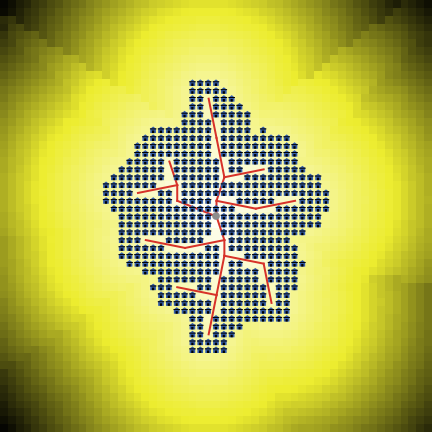
\includegraphics[width=0.29\linewidth]{Figures/CausalityRegimes/ex_60_wdens0_wroad1_wcenter1_seed272727}
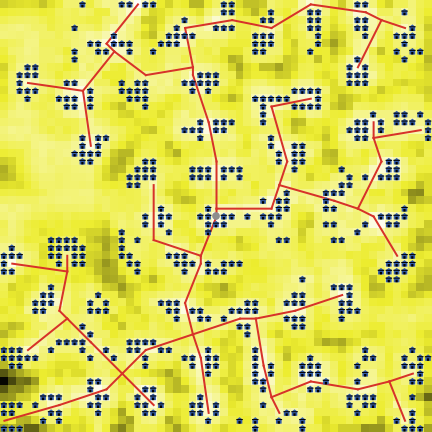
\includegraphics[width=0.29\linewidth]{Figures/CausalityRegimes/ex_60_wdens1_wroad1_wcenter0_seed272727}
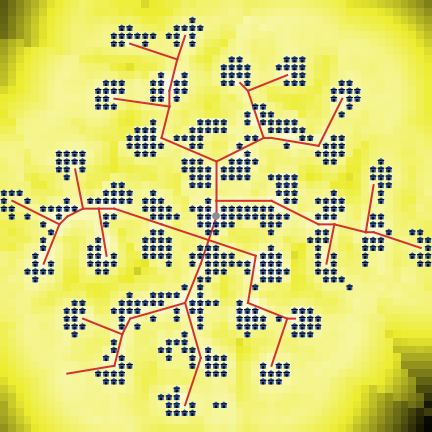
\includegraphics[width=0.29\linewidth]{Figures/CausalityRegimes/ex_60_wdens1_wroad1_wcenter1_seed272727}\\\vspace{0.2cm}
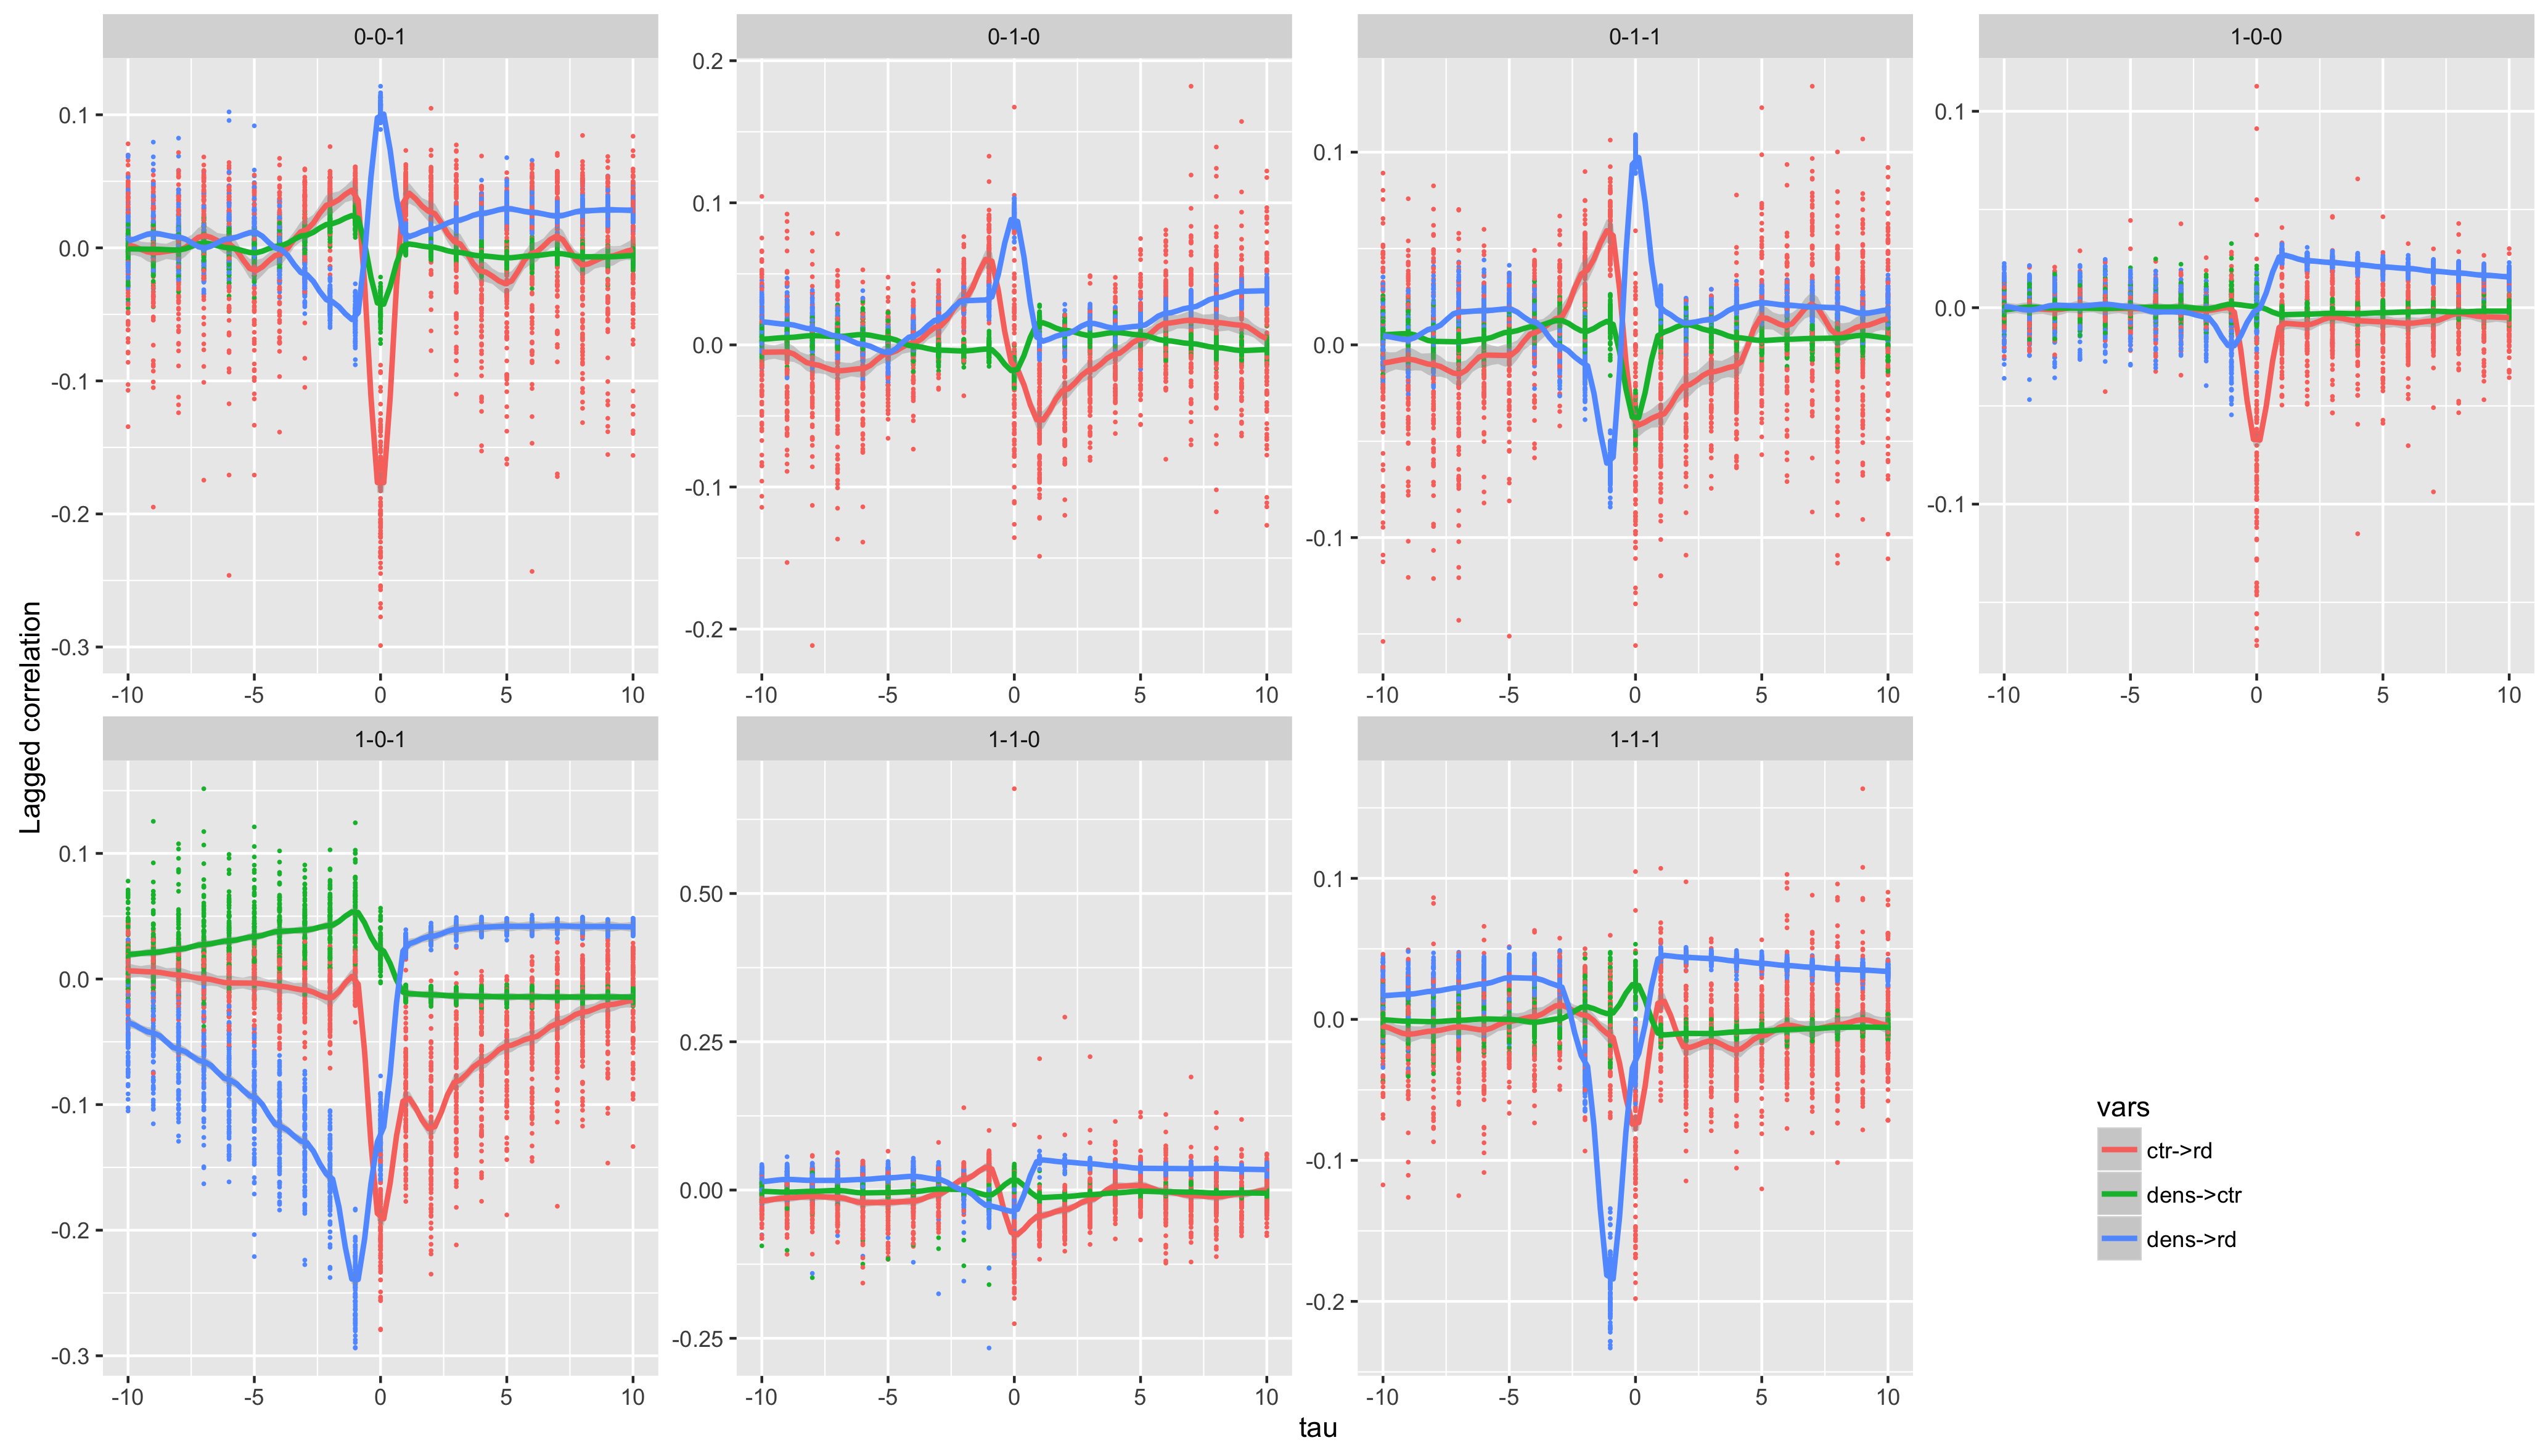
\includegraphics[width=\linewidth]{Figures/CausalityRegimes/laggedcorrs_facetextreme}
\caption[Correlation in the RBD model][Correlations dans le modèle RDB]{Correlation in the RBD model}{\textbf{Correlations dans le modèle RDB} \textbf{(Première ligne)} Exemples de configurations finales variées, obtenues avec $(w_{d},w_{c},w_{r})$ valant respectivement $(0,1,1)$,$(1,0,1)$, et $(1,1,1)$. \textbf{(Deuxième ligne)} Corrélations retardées, pour chaque combinaison des paramètres, en fonction du retard $\tau$. Les différentes couleurs correspondent à chaque couple de variables : distance au centre (\texttt{ctr}), densité (\texttt{dens}) et distance au réseau (\texttt{rd}). Les points montrent l'étendue sur l'ensemble des répétitions du modèle (estimateurs sur $i$ et $t$).}
\label{fig:causalityregimes:exrdb}
\end{figure}
%%%%%%%%%%%%%%%



%%%%%%%%%%%%%%%
\begin{figure}%[h]
\centering
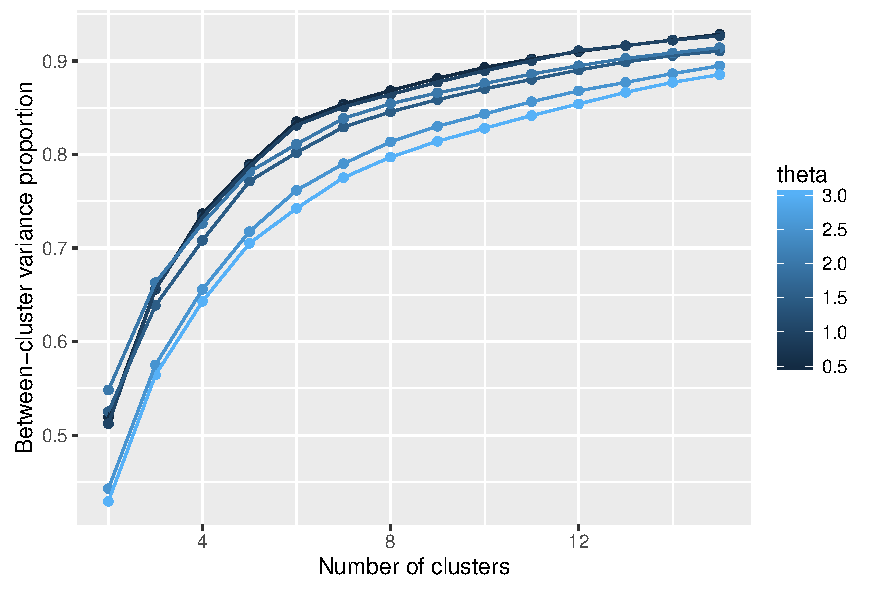
\includegraphics[width=0.49\linewidth]{Figures/CausalityRegimes/ccoef-knum_valuesFALSE_theta05-3.pdf}
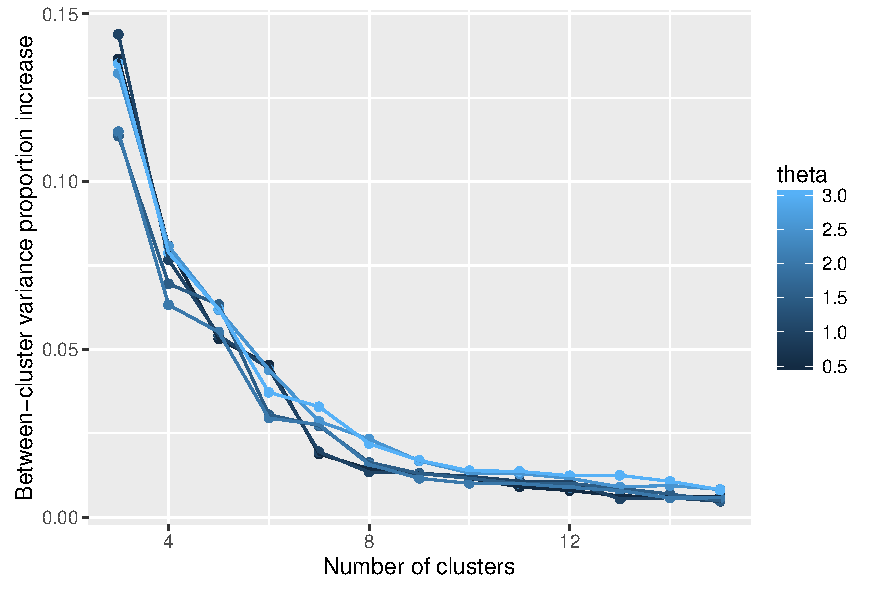
\includegraphics[width=0.49\linewidth]{Figures/CausalityRegimes/dccoef-knum_valuesFALSEtheta05-3.pdf}\\
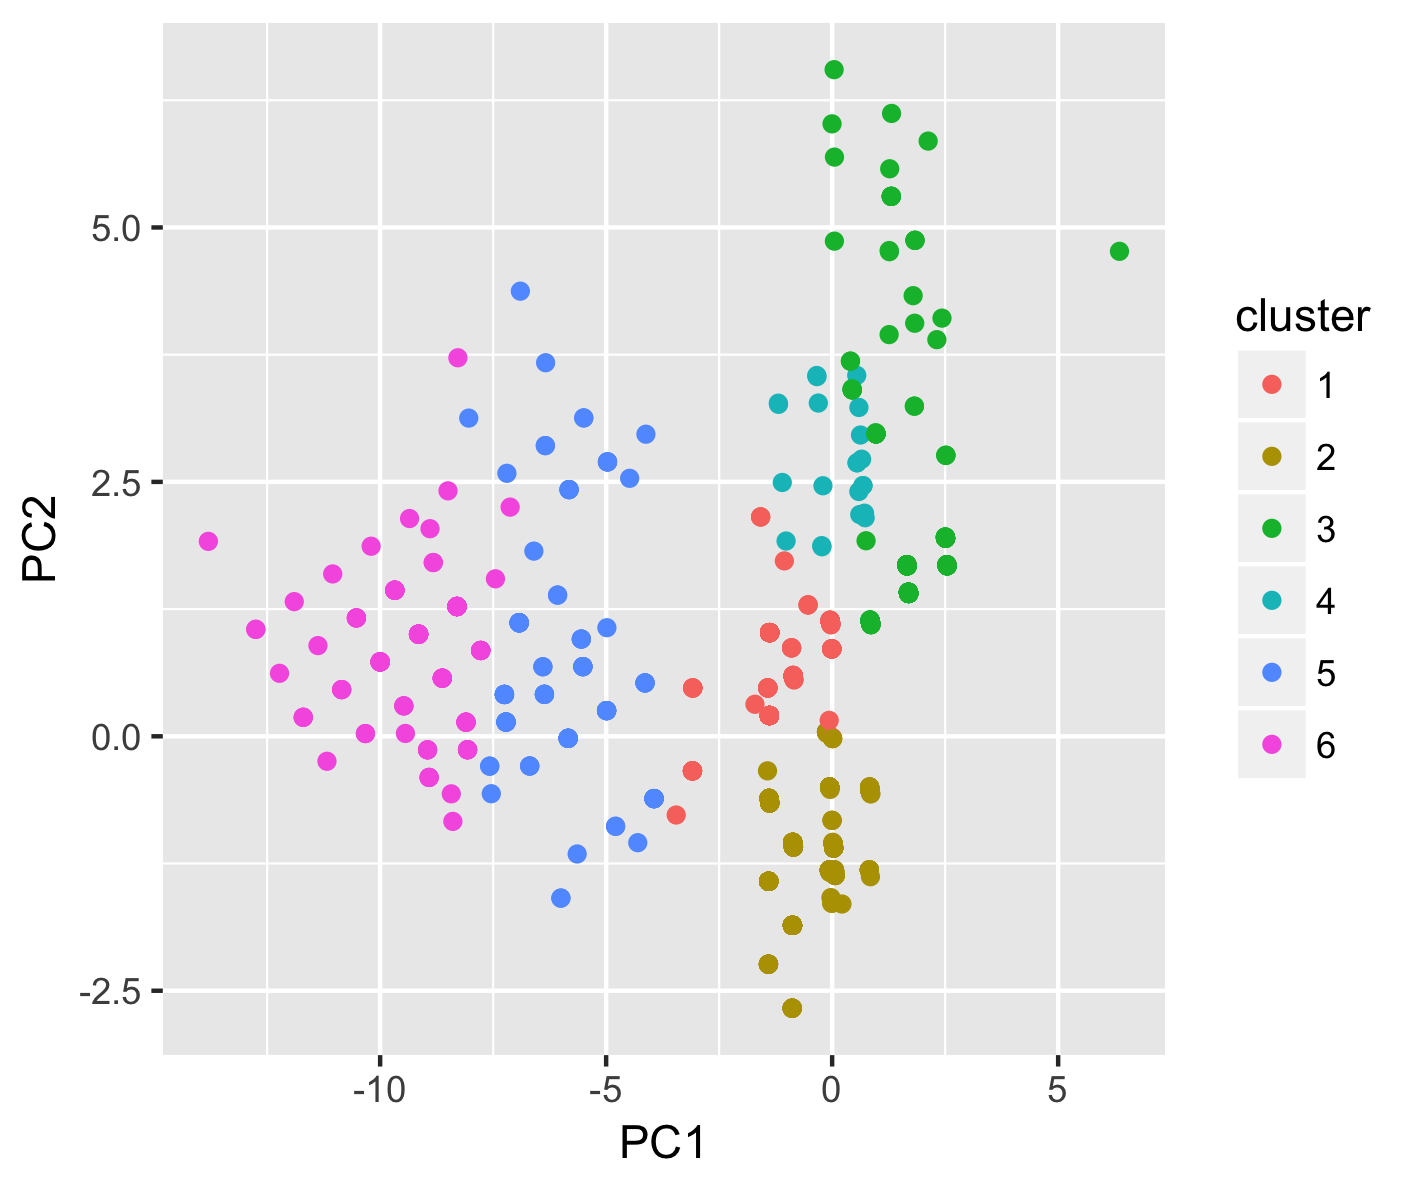
\includegraphics[width=0.29\linewidth]{Figures/CausalityRegimes/clusters-PCA-features_valuesFALSEtheta2_k6}
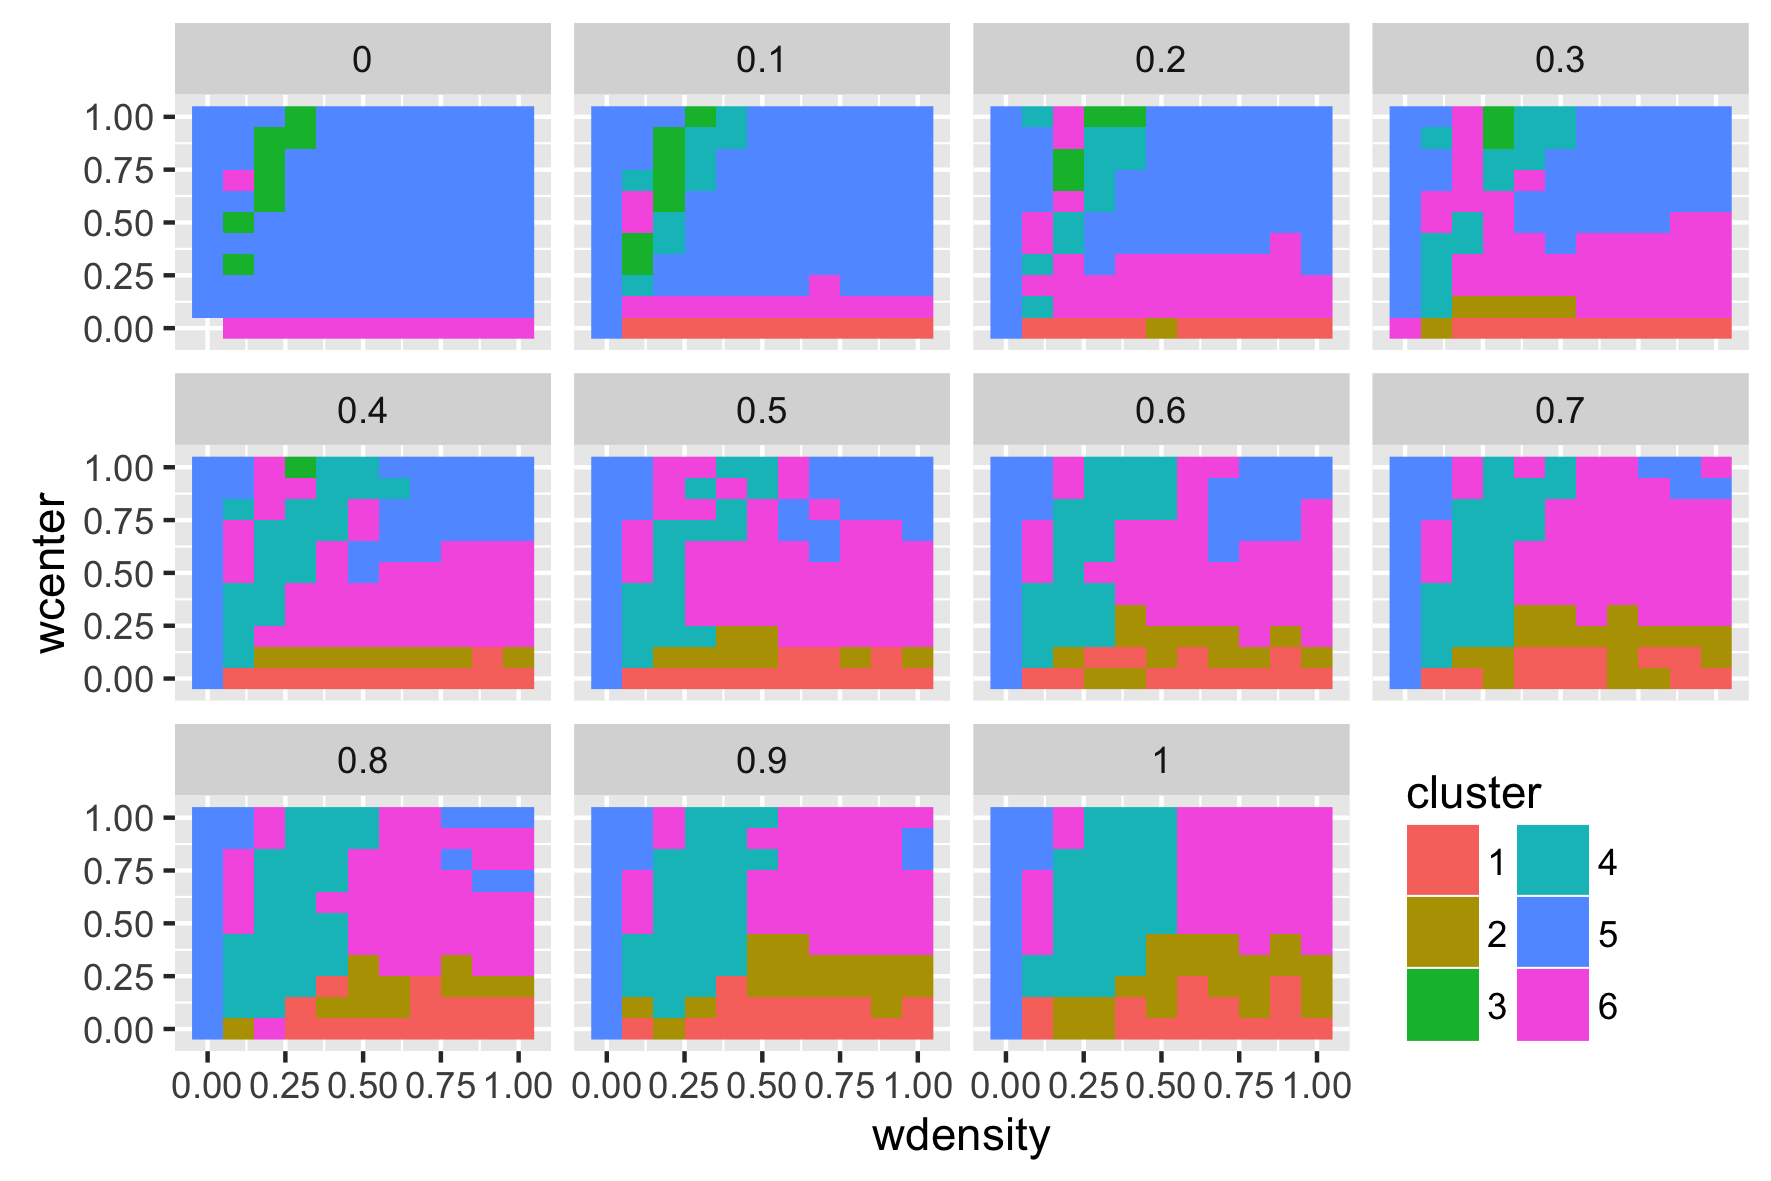
\includegraphics[width=0.69\linewidth]{Figures/CausalityRegimes/clusters-paramfacet_valuesFALSEtheta2_k6}\\
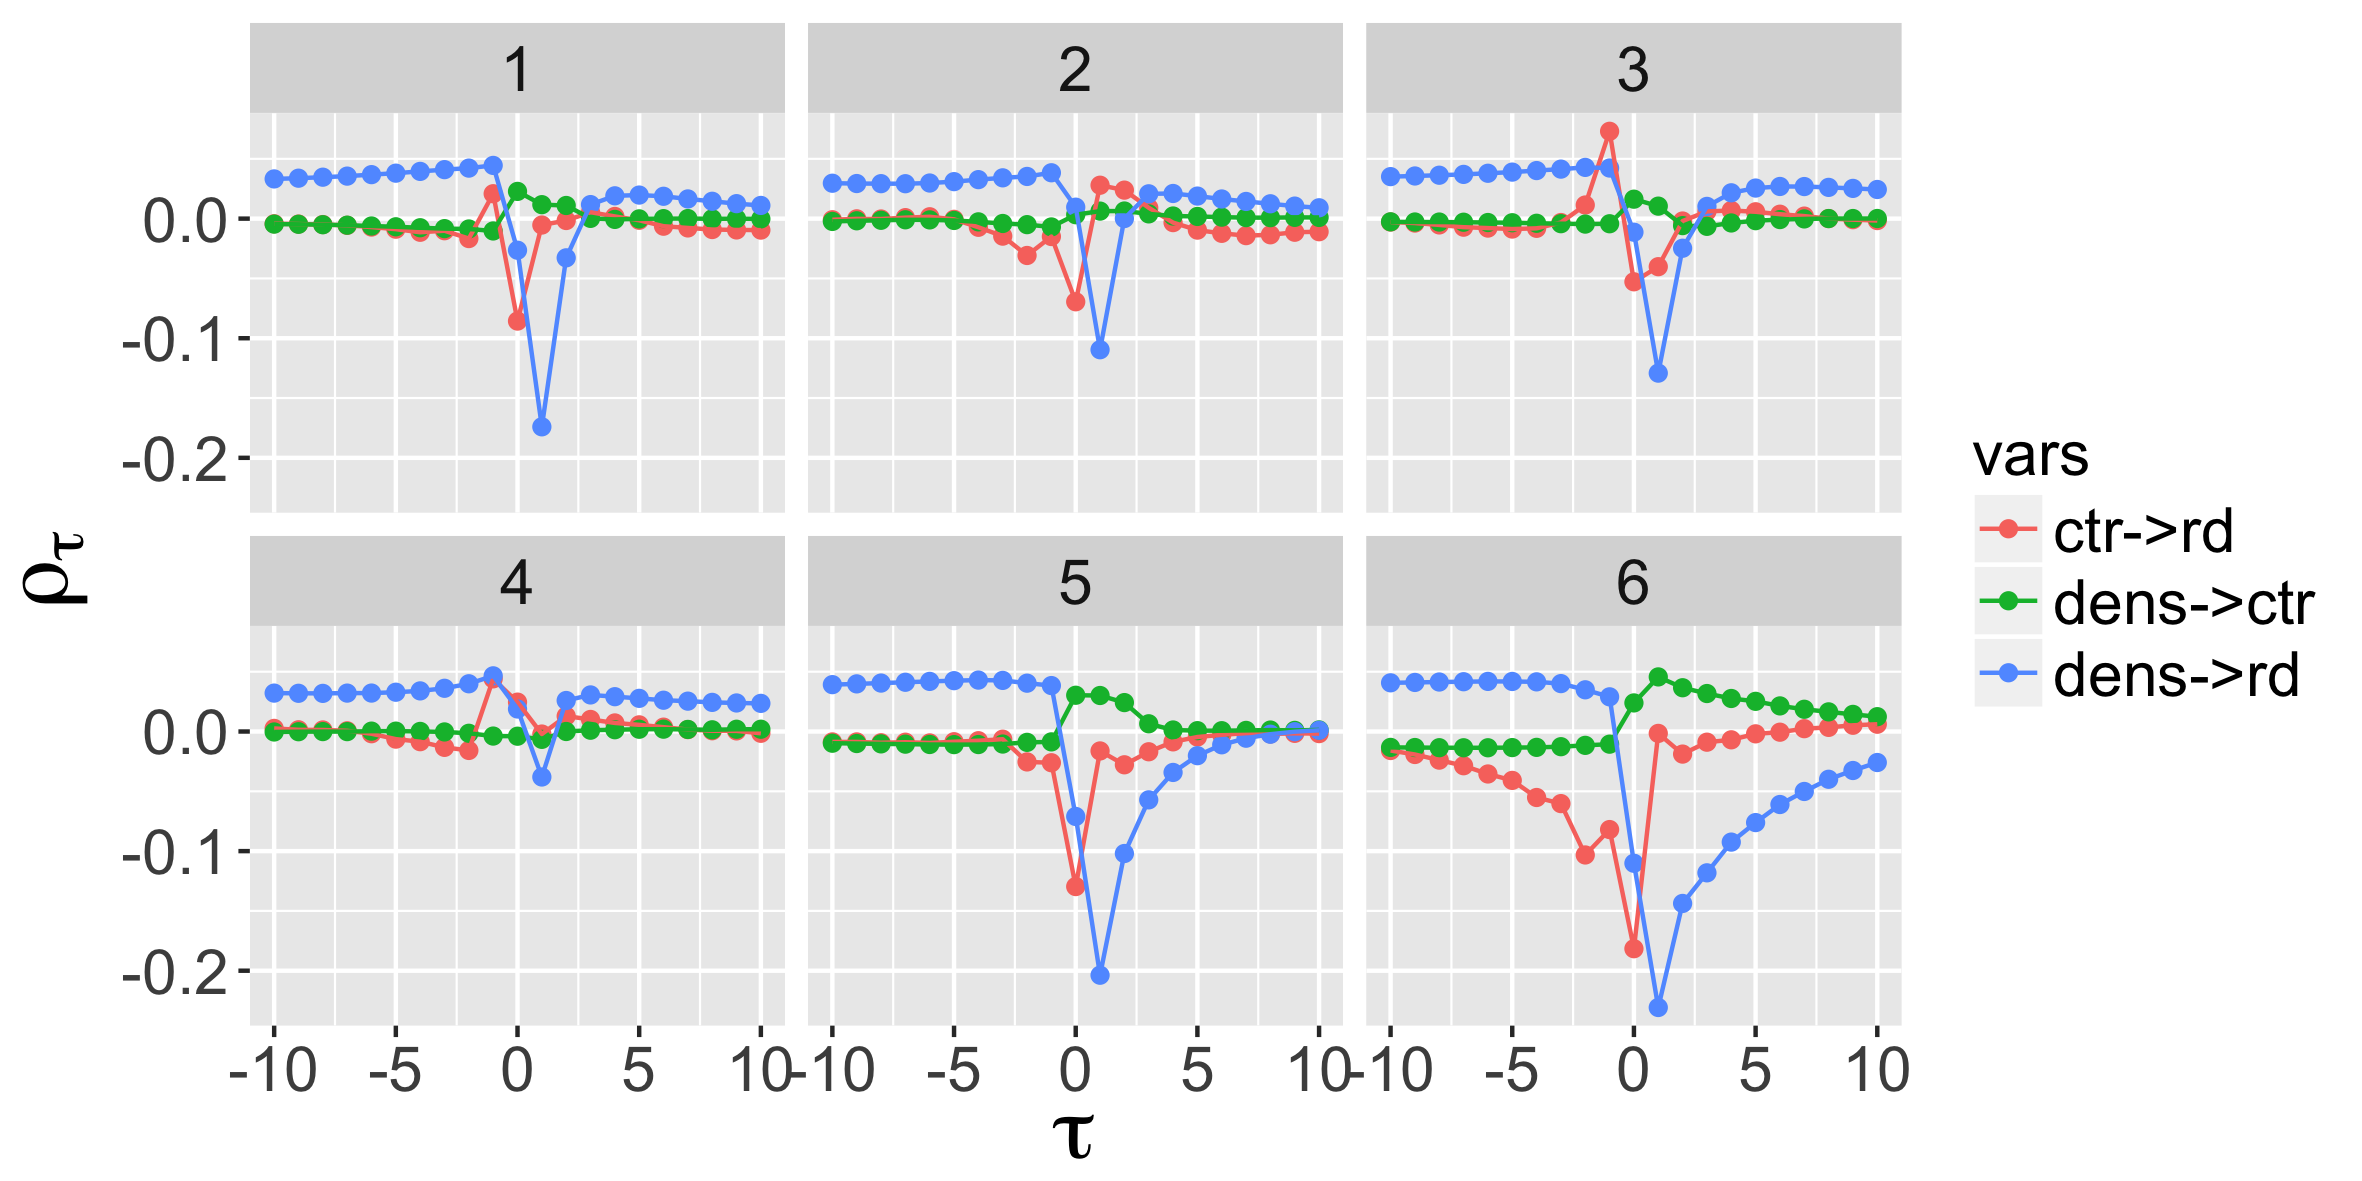
\includegraphics[width=\linewidth]{Figures/CausalityRegimes/clusters-centertrajs-facetclust_valuesFALSEtheta2_k6}
\caption[Identification of interaction regimes][Identification de régimes d'interactions]{Identification of interaction regimes}{\textbf{Identification de régimes d'interactions} \textbf{(Haut Gauche)} Variance inter-cluster comme fonction du nombre de clusters. \textbf{(Haut Droite)} Dérivée de la variance inter-cluster. \textbf{(Milieu Gauche)} \emph{Features} dans un plan principal (81\% de variance expliquée par les deux premières composantes) \textbf{(Milieu Droite)} Diagramme de phase des régimes dans l'espace $(w_{d},w_{c},w_{r})$, $w_r$ variant entre les différents sous-diagrammes de $(w_{d},w_{c}$. \textbf{(Bas)} Trajectoires correspondantes des centroïdes.}
\label{fig:causalityregimes:clustering}
\end{figure}
%%%%%%%%%%%%%%%




Cette méthode doit dans un premier temps être testée et partiellement validée, ce que nous proposons de faire sur des données synthétiques, méthode qui permet une connaissance plus fine des comportements des modèles~\cite{raimbault2016generation}. En écho à l'exemple des relations entre réseaux de transport et territoires qui a permis d'introduire notre problématique précédemment, nous proposons de générer des configurations urbaines stylisées dans lesquelles réseau et densité s'influencent mutuellement, et pour lesquelles les causalités ne sont pas évidents \emph{a priori} étant donné les paramètres du modèle génératif. \cite{raimbault2014hybrid} décrit et explore un modèle simple de morphogenèse urbaine (modèle RBD) répondant parfaitement à ces contraintes. En effet, les variables explicatives de la croissance urbaine, les processus d'extension du réseau et le couplage entre densité urbaine et réseau ne sont pas trop complexes. Cependant, hormis dans des cas extrêmes (par exemple lorsque la distance au centre détermine la valeur foncière uniquement, le réseau dépendra de manière causale de la densité, ou lorsque la distance au réseau seule compte, la causalité sera inversée), les régimes mixtes n'exhibent pas de causalités évidentes : c'est donc un parfait cas pour tester si la méthode est capable d'en détecter. Nous utilisons une implémentation adaptée\footnote{disponible sur le dépôt ouvert du projet à\\\texttt{https://github.com/JusteRaimbault/CityNetwork/tree/master/Models/Simple/ModelCA}} du modèle initial, permettant de capturer les valeurs des variables étudiées pour chaque patch et à chaque pas de temps et de calculer les correlations retardées entre variables au sein du modèle. Nous explorons une grille de l'espace des paramètres du modèle RBD, faisant varier les paramètres de poids de la densité, de la distance au centre et de la distance au réseau\footnote{Le modèle fonctionne de la façon suivante : une valeur des patches est déterminée par la moyenne pondérée de ces différentes variables explicatives, valeur qui détermine la croissance de nouveaux patches à l'instant suivant.}, que l'on note respectivement $(w_{d},w_{c},w_{r})$, dans $\left[0;1\right]$ avec un pas de 0.1. Les autres paramètres sont fixés à leur valeurs par défaut données par \cite{raimbault2014hybrid}. Pour chaque valeur des paramètres, nous procédons à $N=100$ répétitions ce qui est suffisant pour une bonne convergence des indicateurs. Les explorations sont effectuées via le logiciel OpenMole~\cite{reuillon2013openmole}, le grand nombre de simulations (1,330,000) nécessitant l'utilisation d'une grille de calcul. Nous calculons sur l'ensemble des patches les corrélations retardées par estimateur de Pearson non biaisé entre les variations des variables suivantes\footnote{Calculer les corrélations sur les variables directement n'a pas de sens puisque leur valeur n'en a pas en absolu.} : densité locale, distance au centre et distance au réseau. La Fig.~\ref{fig:causalityregimes:exrdb} montre le comportement de $\rho_{\tau}$ pour chaque couple de variable (non dirigé, $\tau$ prenant des valeurs négatives et positives), pour les combinaisons des valeurs extrêmes des paramètres. On peut voir déjà différents régimes émerger : par exemple, $(1,0,1)$ conduit à une causalité de la densité sur la distance au centre avec un retard 1, et une causalité négative de la densité sur la distance au réseau avec le même retard, tandis que distance au centre et au réseau sont corrélés de manière synchrone. Afin d'étudier ces comportements de manière systématique, nous proposons d'identifier des régimes de manière endogène, en procédant à un apprentissage non-supervisé. Nous appliquons une classification des \emph{k-means}, robuste à la stochasticité (5000 répétitions), avec les points caractéristiques (\emph{features}) suivants : pour chaque couple de variable, $\textrm{argmax}_{\tau} \rho_{\tau}$ et $\textrm{argmin}_{\tau} \rho_{\tau}$ si la valeur correspondante est telle que $\frac{\rho_{\tau}-\bar{\rho}_{\tau}}{\left|\bar{\rho}_{\tau}\right|} > \theta$ avec $\theta$ paramètre de seuil, 0 sinon. L'inclusion des \emph{features} supplémentaires des valeurs de $\rho_{\tau}$ n'influence pas significativement les résultats, celles-ci n'ont pas été prises en compte pour réduire la dimension. Le choix du nombre de clusters $k$ est en général épineux dans ce genre de problème~\cite{hamerly2003learning}, dans notre cas le système possède une structure agréable : les courbes de la proportion de variance inter-cluster et de sa dérivée en Fig.~\ref{fig:causalityregimes:clustering}, en fonction de $k$ pour différentes valeurs de $\theta$, présentent une transition pour $\theta = 2$, ce qui donne pour cette courbe une rupture à $k=5$. Un examen visuel des clusters dans un plan principal confirme la bonne qualité de la classification pour ces valeurs. Une classe correspond alors à un \emph{régime de causalité}, dont nous pouvons représenter le diagramme de phase en fonction des paramètres du modèle, ainsi que les trajectoires des centres des clusters (calculées comme barycentre dans l'espace complet initial) en Fig.~\ref{fig:clustering}. Le comportement obtenu est particulièrement intéressant : les régions du diagramme correspondant aux régimes sont clairement délimitées et connexes. Par exemple, on observe l'émergence du régime 6 où la distance au réseau cause fortement la densité de manière négative, mais la distance au centre cause la distance au réseau, régime dont l'étendu maximale sur $(w_d,w_r)$ est pour une valeur intermédiaire $w_r=0.7$. Ainsi, pour maximiser l'impact du réseau sur la densité, il ne faut pas maximiser le poids correspondant, ce qui peut paraître contre-intuitif en premier abord : cela illustre l'intérêt de la méthode dans le cas de relations circulaires difficiles à démêler a priori. Le régime 5, où la distance au réseau influence la densité de la même manière, mais la relation entre distance au centre et route est inversée, est tout aussi intéressant, et est prédominant dans les faibles $w_r$. Le régime 1, extrême, correspond à une situation isolée dans laquelle la distance au centre n'importe pas : cet aspect domine alors totalement les autres processus d'interaction entre densité et réseau. Cette application sur données synthétique démontre ainsi d'une part la robustesse de la méthode vu la cohérence des régimes obtenus, et constitue aussi une qualification beaucoup plus précise des comportements du modèle que celle réalisée dans l'article initial. Dans ce cas précis, il peut s'agir d'un instrument de connaissance des relations entre réseaux et territoires en lui-même, permettant le test d'hypothèses ou la comparaison de processus dans le modèle stylisé.



















%--------------------------------------------------------









%%%%%%%%%%%%%%%%%%%%%%%
\subsection{Network-territory relations in South Africa}{Relations Réseaux-territoires en Afrique du Sud}



\bpar{
We assum that territorial dynamics and network dynamics responded differently to these. We expect to learn from these project informations on interactions at long time scale and large spatial scale, in a very particular context of constrained growth.
}{
Nous démontrons à présent les potentialités de notre méthode sur des données géo-historiques sur le temps long, pour le cas du réseau ferré en Afrique du Sud au cours du 20ème siècle. En faisant l'hypothèse que les territoires et les réseaux réagissent différemment aux événements historiques, les motifs de causalité devraient informer sur leur relations sur le temps long.
}


\subsubsection{Context}{Contexte}


\bpar{
Transportation Networks can be leveraged as a powerful socio-economic control tool, with even more significant outcomes when it percolates to their interaction with territories. The case of South Africa is an accurate illustration, as \cite{baffi:tel-01389347} shows that during apartheid railway network planning was used as a racial segregation tool by shaping strongly constrained mobility and accessibility patterns. In particular, it is shown qualitatively that dynamics between territories and networks profoundly changed at the end of the apartheid, transforming a tool of planed segregation (network shaped was optimized to minimize unwanted accessibility) into an integration tool thanks to recent changes in network topology patterns. We propose to investigate the potential \emph{structural} properties of this historical process, by focusing on dynamical patterns of interactions between the railway network and city growth. More precisely, we try to establish if the segregative planning policies did actually modify the trajectory of the coupled system, what would correspond to deeper and wider impacts. 
}{
Les réseaux de transport peuvent être utilisés comme un puissant outil de contrôle socio-économique, avec des effets encore plus significatifs lorsque ceux-ci perturbent les relations avec les territoires. Le cas de l'Afrique du Sud est une illustration pertinente, puisque \noun{Baffi} montre dans~\cite{baffi:tel-01389347} que lors de l'apartheid la planification du réseau ferré était utilisée comme un outil de ségrégation raciale par l'établissements de motifs de mobilité et d'accessibilité fortement contraints. En particulier, il est montré qualitativement que les dynamiques entre réseaux et territoires ont profondément changé à la fin de l'apartheid, transformant un outil de ségrégation planifiée (une forme de réseau optimisée pour minimisée une accessibilité non désirée) en un outil d'intégration grâce à des changement récents dans la topologie du réseau. Nous étudions ici les potentielles propriétés \emph{structurelles} de ce processus historique, en se concentrant sur les motifs dynamiques des interactions entre le réseau ferré et la croissance des villes. Plus précisément, nous essayons d'établir si les politiques de planification ségrégatives ont effectivement modifié la trajectoire du système couplé, ce qui correspondrait à des impacts plus larges et profonds que leurs effets immédiats.
}


\cite{doi:10.1068/b39089}


\subsubsection{Results}{Résultats}


\paragraph{Data}{Données}


\bpar{
We use a comprehensive database covering the full South African railway network from 1880 to 2000 with opening and closing dates for each station and link, together with a city database spanning from 1911 to 1991 for which consistent ontologies for urban areas have been ensured. These database are described by~\cite{baffi:tel-01389347}, but they are not open so we make available only the aggregated data we used in the analysis.
}{
Nous utilisons une base de données complète couvrant l'ensemble du réseau ferré Sud-Africain de 1880 à 2000 avec les dates d'ouverture et de fermeture pour chaque station et liaison, couplée à une base de données pour les villes s'étendant de 1911 à 1991 pour laquelle des ontologies consistantes pour les aires urbaines ont été assurées. Ces bases de données sont décrites par~\cite{baffi:tel-01389347}, mais ne sont pas ouvertes, nous mettons ainsi à disposition uniquement les données agrégées utilisées dans l'analyse.
}



\paragraph{Network Measures}{Mesures de réseau}

\bpar{
First, a dynamical study of network measures seem to confirm the hypothesis: a trend rupture in closeness centrality (defined for a node as the average travel time to other nodes) at a roughly constant network size evolution, at a date corresponding to the beginning of official segregative policies, suggests that the planning process after this date had in the best case no global effect on network performance, and in the worst case had intended negative effects on accessibility with the aim to physically segregate more.
}{
Une analyse préliminaire consiste à regarder l'évolution dynamique des mesures de réseau, celles-ci pouvant témoigner de ruptures dans les propriétés structurelles du réseau et donc de mutations historiques profondes.
}





\paragraph{Causality patterns}{Motifs de causalité}

We then turn to dynamical interactions between the railway network and city growth. For that, we study Granger causalities, in the large sense of correlations between lagged variables, estimated between cities growth rates and accessibility differentials due to network growth, for all cities and urban areas having a connection to the network.
We test both travel-time and population weighted accessibilities, for varying values of distance decay parameter. Lagged correlations are fitted on varying length time windows, to test for potentially varying stationarity scales.
We find that results are significant with travel-time accessibility only, autocorrelation dominating with weighted accessibility. A time-window of 30 years appears to be a good compromise between the number of significant correlations ($p<0.1$ for a Fisher test) and the absolute correlation level across all lags and distance decays, what should correspond roughly to the time-stationarity scale of the system. We observe furthermore a phase transition when distance decay increases, revealing the shift between the spatial scale of urban areas and the scale of the country, what gives local spatial stationarity scale.
We obtain therethrough clear causality patterns, namely an inversion of the Granger causality (lagged correlation up to 0.5 for several values of distance decay), from accessibility causing population growth with a lag of 10-20 years before the apartheid (1948), to the opposite after the apartheid (lag 20 years). We interpret these as \emph{Structural segregation}, i.e. a significant impact of planning policies on dynamics of interactions between networks and territories. Indeed, the first regime corresponds to direct effect of transportation on migrations in a free context in opposition to the second one. Further work should consist in similar study with more precise socio-economic variables, for example quantifying directly segregation patterns.





\subsubsection{Possible developments}{Développements possibles}


The method of instruments in statistics~\cite{angrist1996identification} is used to identify causal relationships between variables, in a different way than Granger causality test for example. Trying to identify causalities between network dynamics and territorial dynamics is of crucial importance to test our theoretical assumption on the existence of co-evolution.
















